\documentclass[10pt]{beamer}

\usepackage{amssymb,amsthm}% http://ctan.org/pkg/amssymb
\newtheorem{proposition}{Proposition}
\setbeamertemplate{theorems}[numbered]
\usecolortheme[RGB={100,0,0}]{structure}
\setbeamercolor{block title}{use=structure,fg=white,bg=structure.fg!75!black}
\setbeamercolor{block body}{parent=normal text,use=block title,bg=block title.bg!10!bg}

\setbeamertemplate{footline}[frame number]

\usepackage{amsmath}
\DeclareMathOperator*{\argmax}{argmax}
\DeclareMathOperator*{\argmin}{argmin}

\usepackage{natbib}
\bibliographystyle{aea}

\usepackage{xcolor}
\usepackage{graphicx}
\usepackage{amsmath}
\usepackage{numprint}
\npdecimalsign{.}
\nprounddigits{3}
\usepackage{colortbl}
\usepackage{appendixnumberbeamer}
\usepackage{subfigure}
\usepackage{comment}

\usepackage{hyperref}
\usepackage{caption}
\setbeamerfont{caption}{size=\small}
\usetheme{Singapore}
\usecolortheme{beaver}

% for adding regression tables
\usepackage{dcolumn}
% column to line up decimals
\usepackage{booktabs,caption}
\captionsetup[table]{name=Table}
\setlength{\abovecaptionskip}{-1pt}
\setlength{\belowcaptionskip}{-1.5pt}
\usepackage[flushleft]{threeparttable} 
% The above two allow that last line with the dagger as a bottom note.

\usepackage{xcolor}
\definecolor{underbrace}{RGB}{30,199,166}
\newcommand{\textfrac}[1]{
  \begin{tabular}{@{}l@{}}#1\end{tabular}
}
\setbeamertemplate{caption}[numbered]

\title[ERPT]{Exchange Rate Pass-Through and Importers' Credit Constraints: Evidence From China}

\author[Li \& Lu]{Yao Amber LI\inst{*} \and Lingfei LU\inst{*}}

\institute[2024]{\inst{*} \small The Hong Kong University of Science and Technology}

\date{Australasian Trade Workshop (ATW) \\ \vspace{3mm} Christchurch, New Zealand \\ \vspace{4mm} \today }


\begin{document}
	
\begin{frame}
    \maketitle
    \centering
\end{frame}

\AtBeginSection[]
{
    \begin{frame}{Outline}
    \transfade
    \tableofcontents[sectionstyle=show/shaded,subsectionstyle=show/shaded/hide]
    \addtocounter{framenumber}{-1}
    \end{frame}
}

\section{Introduction}

\begin{frame}{What is Exchange Rate Pass-through?}
	\begin{itemize}
		\item Exchange rate shock is a key factor affecting international trade price fluctuations.
		\item The impact of bilateral exchange rate changes on prices denominated in buyers' and sellers' currencies may be asymmetric.
		\item Understanding the pattern of asymmetric prices has important implications for formulating macro policy, including monetary policy, inflation targeting, and the balance of payments.
	\end{itemize}
\end{frame}

\begin{frame}{What is Exchange Rate Pass-through?}
	\begin{itemize}
		\item Exchange rate pass-through (ERPT) is defined as \textbf{the elasticity of local price changes to exchange rate changes}.
		\item Exchange rate pass-through measures how exchange rate risk is shared between buyers and sellers of trade.
	\begin{figure}[htbp]
		\centering
		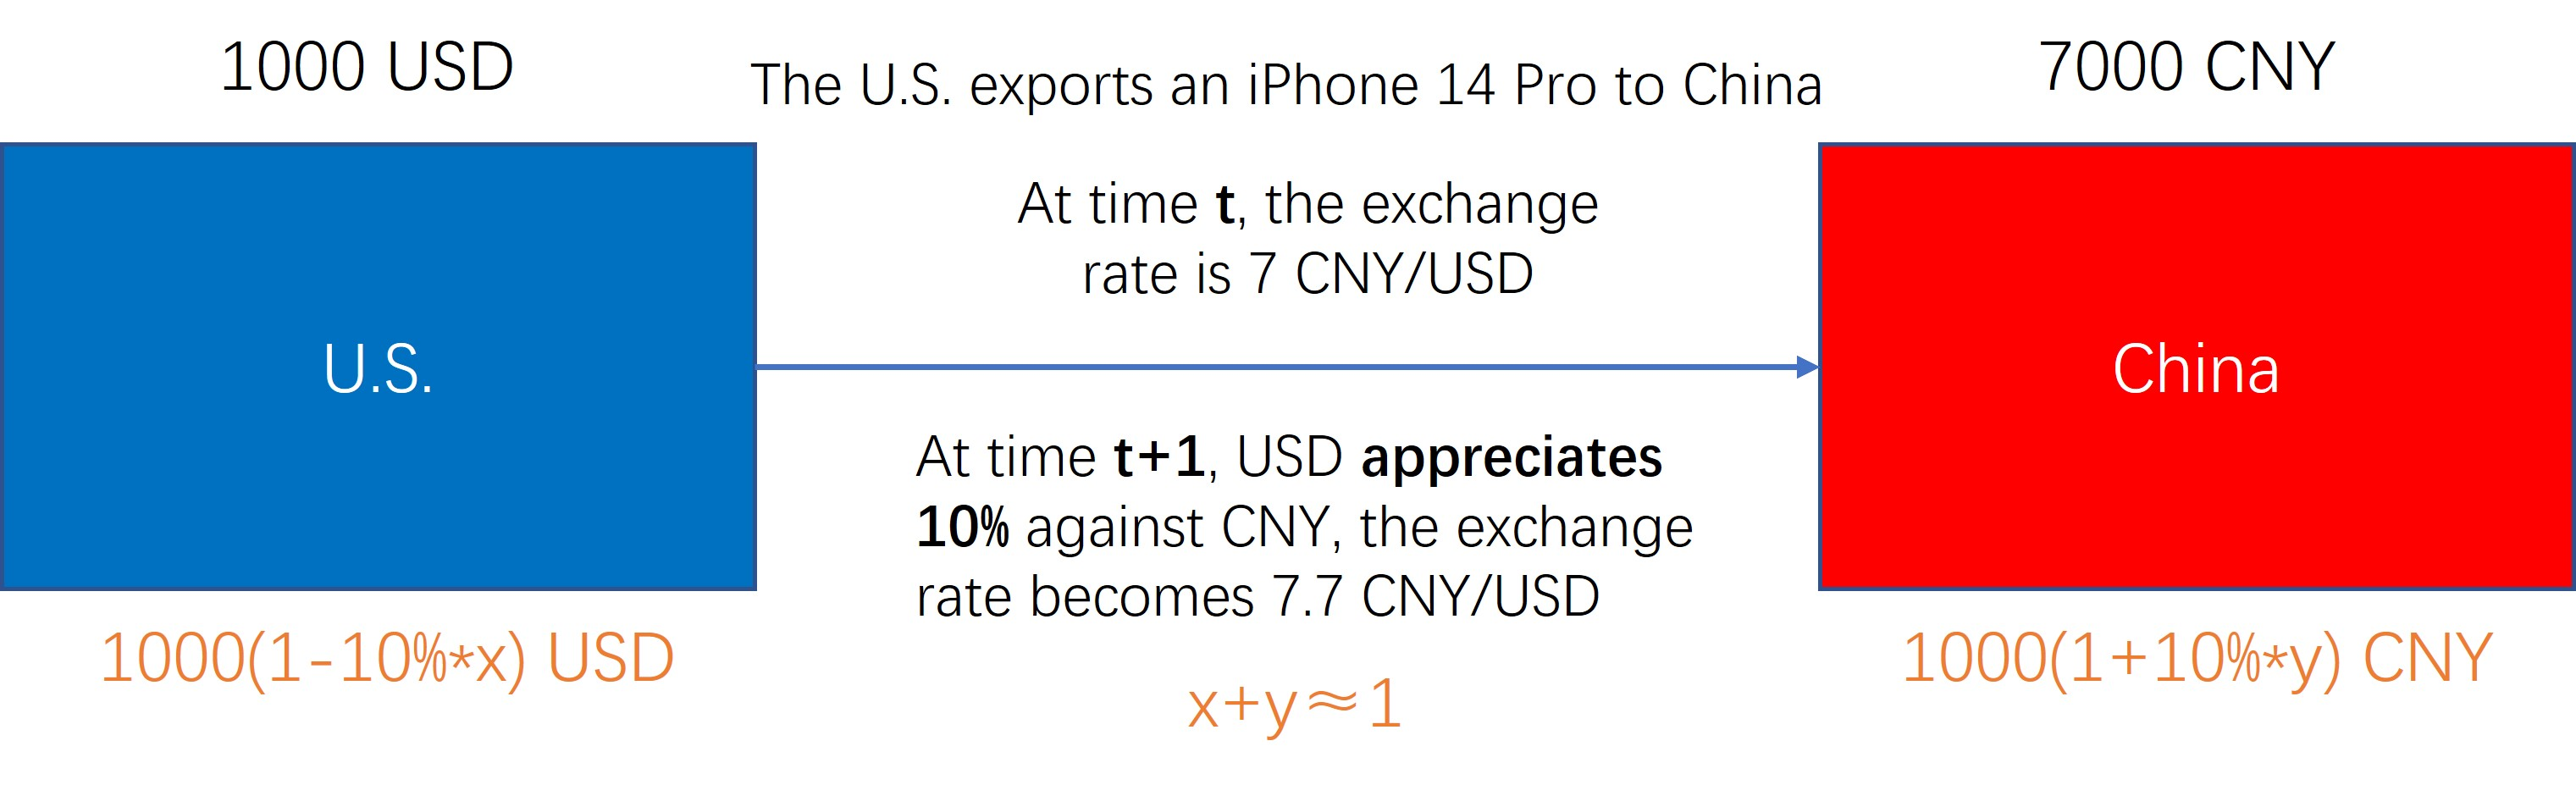
\includegraphics[width=0.9\columnwidth]{ERPT.jpg}
		\label{ERPT}
	\end{figure}
		\item In this example, we call $y$ (or $1-x$) as exchange rate pass-through.
	\end{itemize}
\end{frame}

\begin{frame}{Motivations}
	\begin{itemize}
		\item The degree of exchange rate pass-through can vary significantly from firm to firm. \textbf{But what are the determinants of exchange rate pass-through?}
		\item textbf{The variation in financial constraints across firms and industries could affect international trade} (e.g. \cite{manova2013}).
		\item It remains an open question whether \textbf{importers under financial constraints will behave differently} in price setting during exchange rate fluctuations compared to those less constrained.
	\end{itemize}
\end{frame}

\begin{frame}{Key Questions}
\textbf{Our research questions:}
	\begin{itemize}
		\item [1] What is the difference in exchange rate pass-through (ERPT) patterns between Chinese importers and exporters?
		\item [2] How do importing firms' (buyers') credit constraints affect the exchange rate pass-through?
		\item [3] What are the channels through which credit constraints affect import ERPT? What factors would enhance or mitigate this effect?
	\end{itemize}
\end{frame}

\begin{frame}{What We Do}
Using Chinese customs transaction records and firm-level data, we find:	
	\begin{enumerate}
		\item The average import exchange rate pass-through level in China is significantly less complete than the export one.
		\item Tighter financial constraints of importers will lead exchange rate pass-through to be more complete.
		\item Importers with higher sourcing diversity (who import a certain product from more sources) have a less complete ERPT and are less affected by credit constraints.
	\end{enumerate}	
\end{frame}

\section{Contribution}

\begin{frame}{Contribution: Incomplete Exchange Rate Pass-through}
	\begin{itemize}
		\item We first contribute to the literature on \textbf{exchange rate disconnect}, particularly on firm-level evidence of incomplete price pass-through.
		\item Two milestone papers:
		\begin{itemize}
			\item \cite{bmm2012} (BMM): micro-level evidence of firm heterogeneity in response to real exchange rate shocks.
			\item \cite{aik2014} (AIK): firms with higher import intensity and larger market share have lower ERPT.
			\item More works: \cite{lmx2015}, \cite{chen2016}, \cite{garetto2016}, \cite{auer2016}, \cite{devereux2017}, etc.
		\end{itemize}
		\item Our contribution is to \textcolor{blue}{provide a novel perspective for exchange rate disconnect in emerging economies with immature financial markets}.
	\end{itemize}
\end{frame}

\begin{frame}{Contribution: Credit Constraints and Trade}
	\begin{itemize}
		\item Another important strand of literature discusses \textbf{the effects of firms’ credit constraints on international trade}.
            \begin{itemize}
                \item E.g.: \cite{kroszner2007} \cite{manova2013}, \cite{chaney2016}, \cite{feenstra2015}, \cite{manova-wei-zhang2015}, \cite{fan-lai-li2015}.
            \end{itemize}
		\item For the relationship between credit constraints and exchange rate pass-through, \cite{strasser2013} shows that financially constrained firms tend to pass more exchange rate shocks to prices.
		\begin{itemize}
			\item Two recent articles discussing credit constraints and ERPT with evidence from China, \cite{dai2021} and \cite{xu-guo2021}
		\end{itemize}
		\item We contribute to this literature by \textcolor{blue}{focusing on how importers behave under varying degrees of credit constraints and comparing their heterogeneous capacity to absorb exchange rate shocks}. 
	\end{itemize}	
\end{frame}

\section{Data and Measurements}

\begin{frame}{Data: Customs Transaction Records}
	\begin{itemize}
		\item The first dataset is the transaction level records from the General Administration of Customs of China (GACC) during 2000-2011.
		\begin{itemize}
			\item This dataset provides information on
			all Chinese trade transactions including import and export values, quantities, units, product names and codes, source and destination countries, and type of enterprises.
			\item The categories of products are coded by the Harmonized Coding and Description System (HS) from World Customs Organization (WCO).
		\end{itemize}
		\item We drop unwanted observations referring to \cite{lmx2015}:
		\begin{itemize}
			\item products with inconsistent missing information of unit or quantity
			\item special product categories such as arms (HS2=93), antiques (HS2=97), and special categories (HS2=98 and 99)
			\item transactions existing for only one year without any change over time.
		\end{itemize}
	\end{itemize}
\end{frame}

\begin{frame}{Data: Firm-level Information}
	\begin{itemize}
		\item The second dataset is Chinese Industrial Enterprises (CIE) database from the National Bureau of Statistics of China (NBSC).
		\begin{itemize}
			\item This dataset covers all state-owned enterprises and above-scale firms
			with annual sales of more than 5 million RMB from 1999 to 2007.
			\item The data provide details about firms’ identification code, ownership, industry
			type, and about 80 other variables in the balance sheet including the number of employees, total wage payments, the value of fixed assets, sales income, total operation inputs, etc.
		\end{itemize}
		\item To merge it with customs records, we match the identification codes based on the contact information of firms as in \cite{fan-li-yeaple2015}.
	\end{itemize}
\end{frame}

\begin{frame}{Data: Summary Statistics}
	\begin{itemize}
		\item The summary statistics of the whole customs records, the firm information dataset, and the matched sample are shown as below:
	\end{itemize}
	\begin{figure}[htbp]
		\centering
		\includegraphics[width=0.9\columnwidth]{sumstats1.jpg}
		\label{sumstats1}
	\end{figure}
\end{frame}

\begin{frame}{Data: Exchange Rates and Macro Variables}
	\begin{itemize}
		\item Nominal exchange rates are from Penn World Table (PWT) 10.0 (referring to \cite{feenstra2015}) and consumer price indices (CPI) are from the International Financial Statistics.
		\item The bilateral nominal exchange rate is defined as the number of home currency units that can purchase a unit of foreign currency.
		\item The CPI-based real exchange rate ($RER_{ct}$) is defined as:
		$$
		RER_{ct}=NER_{ct} \cdot \frac{CPI_{ct}}{CPI_{CHN,t}}.
		$$
		\item An increase in $RER_{ct}$ means a real depreciation of the Chinese RMB against the
		foreign country’s $c$ currency.
		\item In addition, we use the real GDP of trading partners from PWT 10.0, computed with national-accounts growth, $RGDP_{ct}$.
	\end{itemize}
\end{frame}

\begin{frame}{Data: Exchange Rates Fluctuations}
		\begin{figure}[htbp]
			\centering
			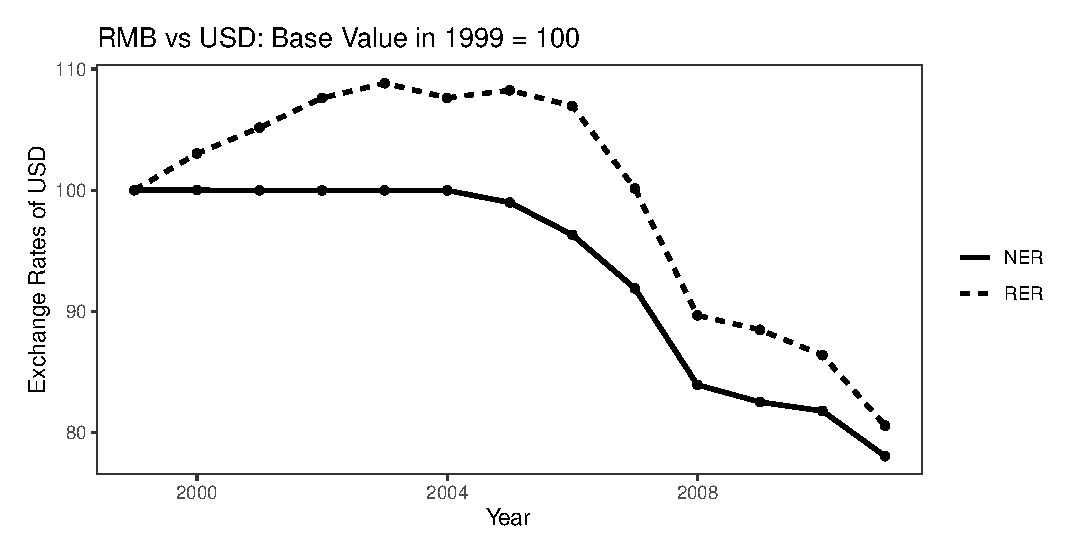
\includegraphics[width=0.7\columnwidth]{R/USD.eps}
			\label{fig.USD}
		\end{figure}
		\begin{figure}[htbp]
			\centering
			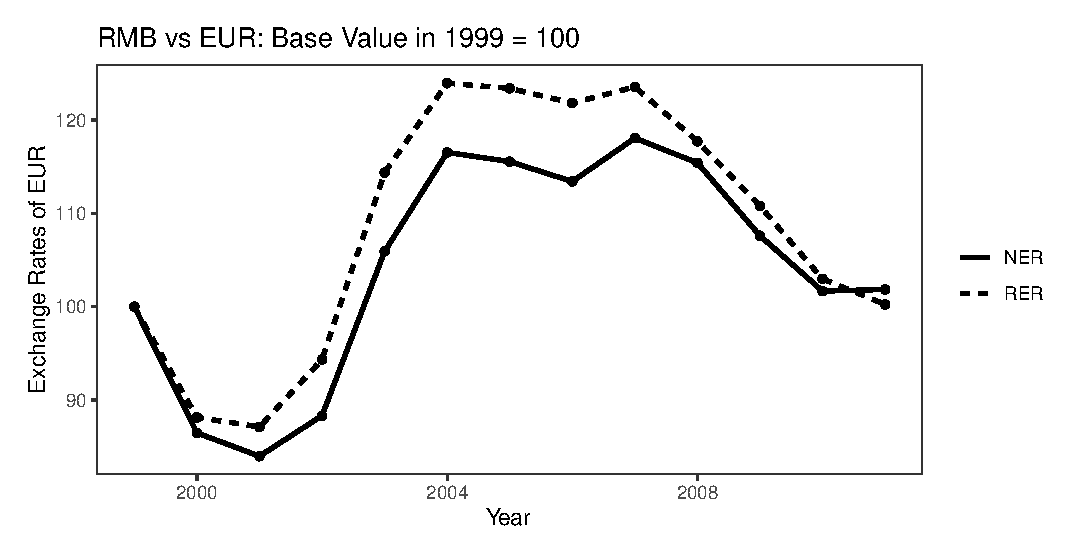
\includegraphics[width=0.7\columnwidth]{R/EUR.eps}
			\label{fig.EUR}
		\end{figure}
\end{frame}

\begin{frame}{Measures of Credit Constraints}
	\begin{itemize}
		\item Following \cite{manova-wei-zhang2015} and \cite{fan-lai-li2015}, we use sector-level financial vulnerability measures to proxy for credit needs (demand for outside capital) and the ability to resist financial risks.
		\begin{enumerate}
			\item \textbf{External Finance Dependence ($ExtFin_j$)}: the share of capital expenditures not financed by operational cash flows.
			\item \textbf{Asset Tangibility ($Tang_j$)}: the share of the net value of tangible assets that firms can pledge as collateral to raise external finance, in its total book value.
			\item \textbf{Inventory-to-sales Ratio ($Invent_j$)}: measure of the production cycle duration and the necessary working capital to maintain inventories and meet demand. 
		\end{enumerate}
		\item We construct the \textbf{first principal component} $FPC_j$ of external finance dependence and asset tangibility as an aggregate measure.
	\end{itemize}
\end{frame}

\begin{frame}{Measures of Credit Constraints}
	\begin{itemize}
		\item Below are the summary statistics of measures of credit constraints using the U.S. and Chinese data.
	\end{itemize}
	\begin{figure}[htbp]
		\centering
		\includegraphics[width=0.9\columnwidth]{sumstats2.jpg}
		\label{sumstats2}
	\end{figure}
\end{frame}

\section{Empirical Analysis}

\begin{frame}{Baseline Estimation Equation}
	\begin{itemize}
		\item The first step goal is to estimate exchange rate pass-through as the elasticity of unit values changes to exchange rate changes.
		\begin{equation}
			\Delta \ln P_{i j c t}=\alpha+\beta \Delta \ln R E R_{c t}+\gamma \Delta \ln R G D P_{c t}+\xi_{i j c}+\tau_{t}+\varepsilon_{i j c t}
			\label{eq4.1}
		\end{equation}
		{\footnotesize where $P_{ijct}$ is the price of the product $i$ bought (sold) by firm $j$ from (to) country $c$ in year $t$.  $\xi_{ijc}$ denotes the firm-product-country level fixed effects. $\tau_t$, the year dummies, control for common macro-shocks across firms.}
		\item To deal with possible non-stationarity, we use the first difference of the logarithms for prices $\Delta \ln P_{i j c t}$, real exchange rates $\Delta \ln R E R_{c t}$ and real GDP $\Delta \ln R G D P_{c t}$ to represent their annual rates of change.
	\end{itemize}
\end{frame}

\begin{frame}{Unit Value as Price}
	\begin{itemize}
		\item The customs records contain trade values (orginally denomicated by US dollars) and quantities $V_{ijct}$, and $Q_{ijct}$ for each HS6 product $i$, each firm $j$, from each country $c$, in each year $t$.
		\item The prices for export and import $P_{i j c t}$ are computed as unit values, both denominated by the Chinese RMB:
		$$
		P_{ijct}=\frac{V_{ijct}\cdot NER_{US,t}}{Q^{D}_{ijct}}
		$$
		\item Because product categories are highly subdivided, we believe that the unit value is an ideal proxy for the transaction price.
	\end{itemize}
\end{frame}

\begin{frame}{Interpretion of Coefficients}
	\begin{itemize}
		\item The coefficient $\beta^{Import}$ measures the completeness of importers' ERPT, i.e. a higher $\beta$ means Chinese importers face more volatile import RMB prices during exchange rate shocks.
		\item However,  $\beta^{Export}$ means the "incompleteness" of exporters' ERPT, i.e. a higher $\beta$ means Chinese exporters pass less exchange rate change to the destination market while having more volatile prices in its domestic currency.
	\end{itemize}
\end{frame}

\begin{frame}{Results: Import Pass-through vs Export Pass-through}
	\begin{figure}[htbp]
		\centering
		\includegraphics[width=0.9\columnwidth]{baseline_import.jpg}
		\label{baseline.imp}
	\end{figure}
\end{frame}

\begin{frame}{Results: Import Pass-through vs Export Pass-through}
	\begin{figure}[htbp]
		\centering
		\includegraphics[width=0.9\columnwidth]{baseline_export.jpg}
		\label{baseline.exp}
	\end{figure}
\end{frame}

\begin{frame}{Finding 1: Import Pass-through vs Export Pass-through}
	\begin{tcolorbox}[colback=blue!5!white, colframe=blue!75!black,title=Key Finding 1]
		\begin{itemize}
			\item The average exchange rate pass-through level for importers in China is less complete than which of exporters.
		\end{itemize}
	\end{tcolorbox}
	\begin{itemize}
		\item For Chineses firms, when RMB depreciates against the currencies of major trading partners, export prices denominated in RMB will rise less significantly than their import prices; when RMB appreciates, export prices in RMB will decrease only to a limited extent, but their import costs will drop more.
		\item For manufacturing firms that are highly dependent on imported intermediate products, the disadvantages of cost increases brought about by depreciation may offset each other with the competitive advantage of export prices.
	\end{itemize}
\end{frame}

\begin{frame}{Estimations with Credit Constraints}
	\begin{itemize}
		\item We study the credit constraint effects on exchange rate pass-through by including an interaction term of sectors’ financial vulnerability:
		\begin{equation}
			\begin{aligned}
				\Delta \ln P_{ijct}=&\alpha+\beta_{1} \Delta \ln RER_{ct}+\beta_{2} \Delta \ln RER_{ct} \cdot FV_{j} \\ &+\gamma \Delta \ln RGDP_{ct}+\xi_{ijc}+\tau_{t} +\varepsilon_{ijct}
			\end{aligned}
			\label{eq.credit}
		\end{equation}
		{\footnotesize where $FV_{j}$ is the financial vulnerability of the sector to which the firm $j$ belongs.}
		\item The interaction coefficient $\beta_2$ represents the effect of industry-level credit constraints on exchange rate pass-through.
		\item The overall ERPT for an importer $j$ is given by $\beta_{1} +\beta_{2} FV_j$ while for an exporter $j$ is given by 1-($\beta_{1} +\beta_{2} FV_j)$.
	\end{itemize}
\end{frame}

\begin{frame}{Results: Effects of Credit Constraints}
	\begin{figure}[htbp]
		\centering
		\includegraphics[width=0.8\columnwidth]{credit_import.jpg}
		\label{credit.imp}
	\end{figure}
\end{frame}

\begin{frame}{Results: Effects of Credit Constraints}
	\begin{figure}[htbp]
		\centering
		\includegraphics[width=0.8\columnwidth]{credit_export.jpg}
		\label{credit.exp}
	\end{figure}
\end{frame}

\begin{frame}{Finding 2: Effects of Credit Constraints}
	\begin{tcolorbox}[colback=blue!5!white, colframe=blue!75!black,title=Key Finding 2]
		\begin{itemize}
			\item Tighter financial constraints of importers will lead exchange rate pass-through to be more complete.
		\end{itemize}
	\end{tcolorbox}
	\begin{itemize}
		\item Exchange rate fluctuations are more likely to be reflected in unstable import costs for importers in financially vulnerable industries because they have weak bargaining power in the international market.
		\item \textit{Credit constraints expose Chinese manufacturing firms to greater exchange rate risk in international trade.}
	\end{itemize}
\end{frame}

\begin{frame}{Additional Firm-level Factors}
	To answer the third question, we introduce a vector $\mathbb{Z}_{jt}$ (or its lagged form $\mathbb{Z}_{jt-1}$) to include additional factors which may affect ERPT.
	\begin{enumerate}
		\item \textbf{Sourcing Diversity}: defined as the number of source countries from which an importer $j$ imports a certain HS6 product type $i$. 
		\item \textbf{Markup}: estimated by the GMM method following \cite{dlw2012} and \cite{bkl2021}.
		\item \textbf{Market Share}: defined as a firm’s value share in the import market, within a given HS6 product category.
		$$
		S^{D}_{ijct} \equiv \frac{v^{D}_{ijct}}{\sum_{j^{\prime} \in J_{ict}} v^{D}_{ij^{\prime}ct}}
		$$
	\end{enumerate}
\end{frame}

\begin{frame}{Estimations with Additional Factors}
	\begin{itemize}
		\item Estimation equations with additional factors $\mathbb{Z}_{jt}$:
		\begin{equation}
			\begin{aligned}
				\Delta \ln P_{ijct}=&\alpha+[\beta_{1}+ \beta_{2} \cdot FV_{j}+\beta_{3} \cdot {\mathbb{Z}_{jt}}'] \Delta \ln RER_{ct} \\&+\gamma \Delta \ln RGDP_{ct}+ {\mathbb{Z}_{jt}}' \eta+\xi_{ijc}+\tau_{t} +\varepsilon_{ijct}.
			\end{aligned}	
			\label{eq.add.control}
		\end{equation}
		\begin{equation}
			\begin{aligned}
				\Delta \ln P_{ijct}=&\alpha+[\beta_{1}+ \beta_{2} \cdot FV_{j}+\beta_{3} \cdot {\mathbb{Z}_{jt}}'+\beta_{4} \cdot FV_{j} \cdot {\mathbb{Z}_{jt}}'] \Delta \ln RER_{ct} \\ &+\gamma \Delta \ln RGDP_{ct}+ {\mathbb{Z}_{jt}}' \eta+\xi_{ijc}+\tau_{t} +\varepsilon_{ijct}.
			\end{aligned}	
			\label{eq.add.interaction}
		\end{equation}
		\item Now we will focus on how sourcing diversity affects exchange rate pass-through for firms subject to different levels of credit constraints.
	\end{itemize}
\end{frame}

\begin{frame}{Results: Sources, Credit Constraints, and ERPT}
	\begin{figure}[htbp]
		\centering
		\includegraphics[width=0.95\columnwidth]{source1.jpg}
		\label{source1}
	\end{figure}
\end{frame}

\begin{frame}{Results: Sources, Credit Constraints, and ERPT}
	\begin{figure}[htbp]
		\centering
		\includegraphics[width=0.95\columnwidth]{source2.jpg}
		\label{source2}
	\end{figure}
\end{frame}

\begin{frame}{Results: Sources, Credit Constraints, and ERPT}
	\begin{figure}[htbp]
		\centering
		\includegraphics[width=0.95\columnwidth]{source_distance.jpg}
		\label{source.distance}
	\end{figure}
\end{frame}

\begin{frame}{Finding 3: Sourcing Diversity, Credit Constraints, and ERPT}
	\begin{tcolorbox}[colback=blue!5!white, colframe=blue!75!black,title=Key Finding 3]
		\begin{itemize}
			\item Importers with a wider sourcing base (who import a certain product from more sources) have a less complete ERPT and are less affected by credit constraints.
		\end{itemize}
	\end{tcolorbox}
	\begin{itemize}
		\item If a firm can import the same product from more sources, it has more flexibility to escape the unfavorable exchange rate risk.
		\item A more diverse importer can either switch from one source to another to reduce costs (trade diversion effect), or make a more credible threat to negotiate a more stable price.
	\end{itemize}
\end{frame}

\section{Robustness}

\begin{frame}{Robustness 1: Alternative Measures of Credit Constraints}
	\begin{itemize}
		\item We use alternative credit constraint measures from Chinese data.
	\end{itemize}
	\begin{figure}[htbp]
		\centering
		\includegraphics[width=0.8\columnwidth]{robust_cn.jpg}
		\label{robust.cn}
	\end{figure}
\end{frame}

\begin{frame}{Robustness 2: Alternative Transaction Samples}
	\begin{itemize}
		\item We exclude USD-pegged countries since the nomial exchange rates of RMB/USD were stable until 2004 due to the pegging scheme.
	\end{itemize}
	\begin{figure}[htbp]
		\centering
		\includegraphics[width=0.75\columnwidth]{robust_nopeg.jpg}
		\label{robust.nopeg}
	\end{figure}
\end{frame}

\begin{frame}{Robustness 3: Trade Type Controls}
	\begin{itemize}
		\item Robustness check 3: we add controls of (1) two-way traders vs pure importers, (2) ordinary trade vs processing trade.
	\end{itemize}
	\begin{figure}[htbp]
		\centering
		\includegraphics[width=\columnwidth]{robust_type.jpg}
		\label{robust.type}
	\end{figure}
\end{frame}

\begin{frame}{Firm Heterogeneity in Markup and Market Share}
	\begin{itemize}
		\item Will firms with higher markup have less complete exchange rate pass-through?
		\item Do credit constraints still have significant effect on exchange rate pass-through after controlling for markup?
		\item How an importer's market share in a specific product market affects its exchange rate pass-through?		
	\end{itemize}	
\end{frame}

\section{Conclusion}

\begin{frame}{Conclusion}
	\begin{itemize}
		\item In this paper, we provide evidence at a disaggregated level for the incomplete import exchange rate pass-through in China and reveal how importers’ financial constraints affect the pass-through.
		\item We find that:
		\begin{enumerate}
			\item The average import exchange rate pass-through in China is around 70\%, which is less than the 95\% level for export pass-through.
			\item Both import and export exchange rate pass-through are more complete for firms in industries with tighter credit constraints.
			\item Import source diversity can effectively reduce import price pass-through and offset the effects of credit constraints.
		\end{enumerate}
		\item In the future, we need to explore the underlying mechanism by which credit constraints affect exchange rate pass-through. 
	\end{itemize}
\end{frame}

\begin{frame}[allowframebreaks]
	\frametitle{References}
	\bibliographystyle{apalike}
	\footnotesize
	\bibliography{ref.bib}
\end{frame}
	
\end{document}